\documentclass[conference]{IEEEtran}

\hyphenation{op-tical net-works semi-conduc-tor}

\usepackage[dvipdfmx]{graphicx}


\begin{document}

\title{移植可能性に着目した再利用によるJavaテストコード自動生成に向けた調査}

\author{\IEEEauthorblockN{Kinari Nishiura}
\IEEEauthorblockA{Kyoto Institute of Technology\\
Email: k-nishiura@se.is.kit.ac.jp}}

\maketitle

\begin{abstract}
Software developers test their software products to keep the quality high.
Automated testing with test codes lightens their efforts to test.
However, writing appropriate test codes manually is difficult and a time-consuming activity.
Some existing techniques to automatically create test codes require to prepare a detailed material like a natural language specification.
Otherwise, they can only create very simple unit test with poor quality.
An approach which reuses test codes from other projects has a possibility to improve above problems. 
However, the process of transportation and modification of test codes has not been automated yet.

In this work we research Java OSS projects with test codes to assess the feasibility of an automatic test codes generation technique based on reuse from other projects.


\end{abstract}

\IEEEpeerreviewmaketitle



\section{Introduction}
ソフトウェアの品質を高く保つことは広く要求されている。
例えばリリース後にソフトウェアの不具合が明らかになった場合、ユーザの安全への脅威や経済的損失の発生、加えて開発者に対するユーザの信頼低下を招く恐れがある。
これを抑制するため、ソフトウェアの不具合をリリース前に検出するソフトウェアテストが広く行われている。

かつてのソフトウェア開発では、全てのテストは手動による入力および出力の目視確認によって行われていた。
この労力を軽減すべく、テストを行うためのプログラムを記述するテストコードが作成されるようになった\cite{Klammer2017}。
テストコードには通常、テスト対象プログラムへの入力あるいは操作とその期待出力が記述され、実際の出力と期待出力を照合することで動作が正しく行われているかを確認する。
開発者はテストコードを作成し実行することで自動的に何度でもテストを行うことができ、ソフトウェアテストに伴うコストを軽減できる\cite{Orso2014}。

こうした自動テストを支援する様々な技術が生まれている。
例えばJavaの単体テストフレームワークであるJUnitを使用することで関数単位のテストコードを簡潔に記述することができる\cite{JUnit}。
また、Eclipse等のIDEではテストフレームワークによって記述されたテストを自動的に検出でき、開発者によるテストを行いやすくしている\cite{Eclipse}。
Maven等のビルド管理ツールではビルド時にテストコードによるテストを自動的に実行することができる[要引用]。
またこれを利用して、リモートリポジトリへのコミット時に自動的にテストを実行でき、製品を常に動作可能な状態に保つ継続的インテグレーション(CI)ツールも存在している\cite{TravisCI}。
他にも、テストコードを先に作成してから製品の開発を始めるテスト駆動開発(TDD)や振る舞い駆動開発(BDD)と呼ばれるプラクティスも提案されている[要引用]。

一方で、テストコードの記述は基本的には手動で行われている。テストコードの記述作業は時間的なコストが高く、メンテナンスコストや学習コストの高さとも相まって自動テストを導入する大きな障害となっている[要引用]。
また、テストコード記述の作業コストの高さは開発者の過労働やテスト漏れによるリリース後の不具合発生を誘発させている[要引用]。
テストコードの自動生成技術はこれらの問題を解決しうる。

テストコードの自動生成を目的とした研究がいくつか断片的に成されている。
EvoSuiteはいくつかの選択可能な基準で最適化された関数単位でのテストコードを自動的に生成することができる\cite{Fraser2013, Almasi2017}。
しかし、ソースコードの質が低いことが指摘されている\cite{Shamshiri2018}。
また、単一の関数を対象としたごく簡単なテストシナリオにしか対応していない。
他にも、BDDにおける製品の振る舞いを中間言語で記述したファイルや、JavaDocなどの構造化された自然言語で書かれた仕様書からテストコードを自動生成する手法がいくつか提案されている\cite{Motwani2019, JBehave}。
しかし、これらのアプローチにはテストコードの原型となる文書の準備を要するため、純粋な自動生成とは言い難い。
深層学習によってソースコードを自動生成するプログラム合成のような技術をテストコードに適用した研究は現時点では確認できない。
またプログラム合成は研究用に定義されたドメイン固有言語を対象にしているものが多く、あるいはコード生成の精度が十分でないなど、実用的なテストコード生成への見通しが悪い[要引用]。

一方、既存のコードを再利用することで開発効率や信頼性が向上することが一般に知られている[要引用]。
このことから、既存のプロジェクトに存在するテストケースを再利用するアプローチは実用性の上でも効果的であると期待できる。
SondhiらはJavaおよびPythonのオープンソースライブラリのテストコードの再利用性について調査し、類似した機能へのテストコードが存在することや、テストコードを移植することで同様のテストが行えることを示した\cite{Sondhi2019}。
ただし、あるライブラリのテストコードを別のライブラリに適用する際には手動で書き換えを行っている。
このことから、テストコードの移植可能性には未だ制限がある。

既存のプロジェクトのテストコードを別のプロジェクトに移植する際の課題について、我々は以下のように考える。
まず、移植したテストコードが移植先のプロジェクトの機能を正しくテストできるか? 
この質問はテストコードの移植の成功を前提としているため、現時点では答えられない。
ただ、移植したテストコードが正しくテストを行うためには、そのテストコードが移植先においても実行可能な状態にする必要がある。
では、移植したテストコードを移植先のプロジェクトに対して適切に動作するよう改変できるか? 
テストコードの実装はテスト対象の実装に依存するため、同様の機能を提供していてもその実装が異なる場合、テスト内容を保ったまま適切に複雑な改変を施すのは困難であると考える。
であるならば、再利用のために移植するテストコードの持つべき条件とは何か? 
それは機械的な処理を施すだけで、移植先のプロジェクトにおいても実行可能となるような実装を持つことであると考える。

本研究では、再利用ベースのテストコード自動生成技術の提案に向けた、既存プロジェクトの持つテストコードの移植可能性について調査する。
調査対象にはGitHub上に存在するテストコードを持つJavaオープンソースシステム(以下、OSS)プロジェクトを用いた。
Javaは実装言語としても研究対象言語としても広く使われており、GitHubに多くのOSSプロジェクトが登録されている点や、テストフレームワークとしてJUnitが広く使用されている点を考慮して選択された。

また本研究では、あるテストメソッドを別のプロジェクトに移植できる条件を提案する。
これはテストメソッド中で呼び出されるテスト対象のメソッドについて、それらの引数および返り値の型が同一であるメソッドが全て存在し、かつメソッドとクラス間の関係が保たれていれば、そのオペレーションが移植後でも行えるという理屈に基づいている。
移植可能性を満たすテストメソッドは、そこで呼び出される補助メソッドとともに、対応する識別子の変更などを行ったのち一つのテストコードとして移植できることが期待される。

本研究の目的は、我々の提案する移植可能条件を満たすテストコードがどの程度存在し、移植可能なテストコードが実際に移植先でどの程度テストを行えるかを明らかにすることである。
加えて、プロジェクトの属するドメインや用意する移植元プロジェクトの数が結果に与える影響を調べる。
また調査結果をもとに、再利用によるJavaテストコード自動生成技術の実現可能性を考察する。

\begin{description}
\item[RQ1] テストコードの移植元として使用できるプロジェクトはどの程度存在するか?
\item[RQ2] テストメソッドの持つ他のメソッドへの結びつきはどの程度存在するか?
\item[RQ3] 移植可能性を満たすテストメソッドはどの程度存在するか?
\item[RQ4] 移植されたテストコードはどの程度有効か?
\end{description}

調査の結果、(調査結果)が示された。

本論文の以降の構成を示す。
二章では調査対象であるテストコードの構造について詳述する。
三章では提案するテストコードの移植可能条件について述べる。
四章ではそれぞれの研究設問について実際に調査し、調査結果を述べる。
五章ではそれをもとに再利用によるテストコード自動生成技術について議論する。
六章では妥当性への脅威について述べる。
七章では関連研究を紹介し、
八章で結言と今後の課題を述べる。

\section{テストコードの構造}

\begin{figure*}[tb]
\begin{center}
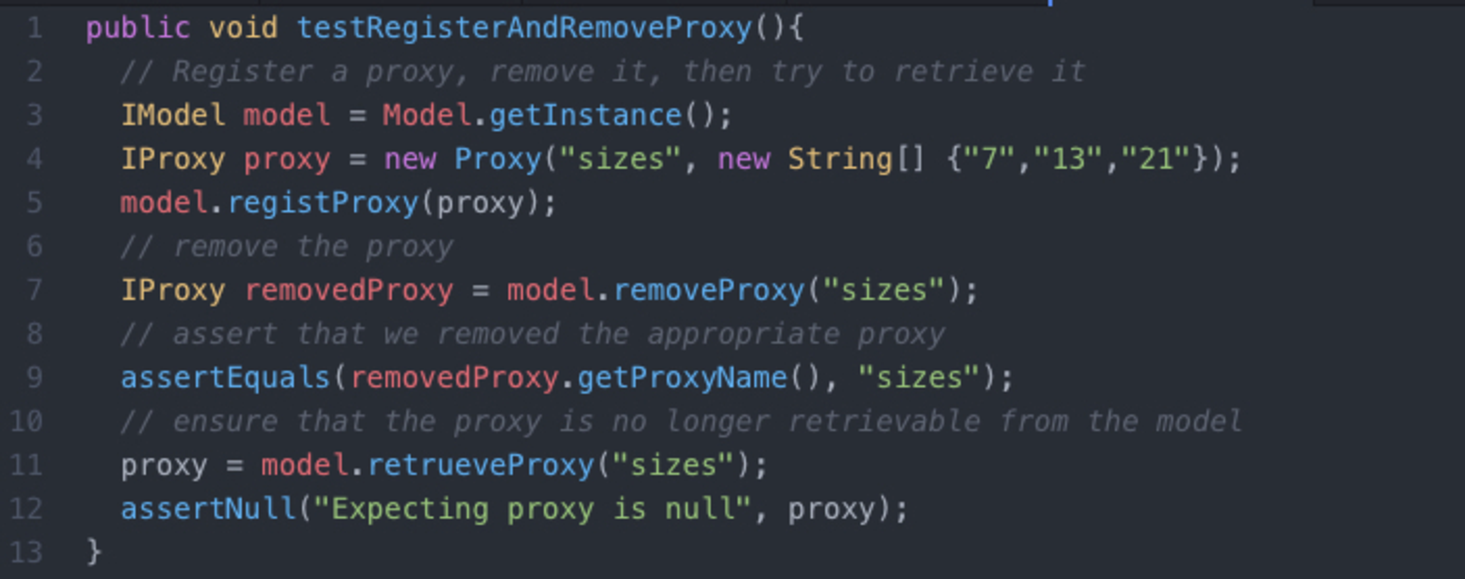
\includegraphics[width=14cm]{img/snipetA.pdf}
\caption{単純なテストコード例}
\label{snipetA}
\end{center}
\end{figure*}

テストフレームワークとしてJUnitを用いたものを例に挙げて説明する。
単純な単体テストの例として、pureMVC\footnote{http://puremvc.org}のあるテストコードスニペットを\ref{snipetA}に示す。
このスニペットは関連研究\cite{Ghafari2017}でも例として使用されている。
ここでは、



\begin{figure*}[tb]
\begin{center}
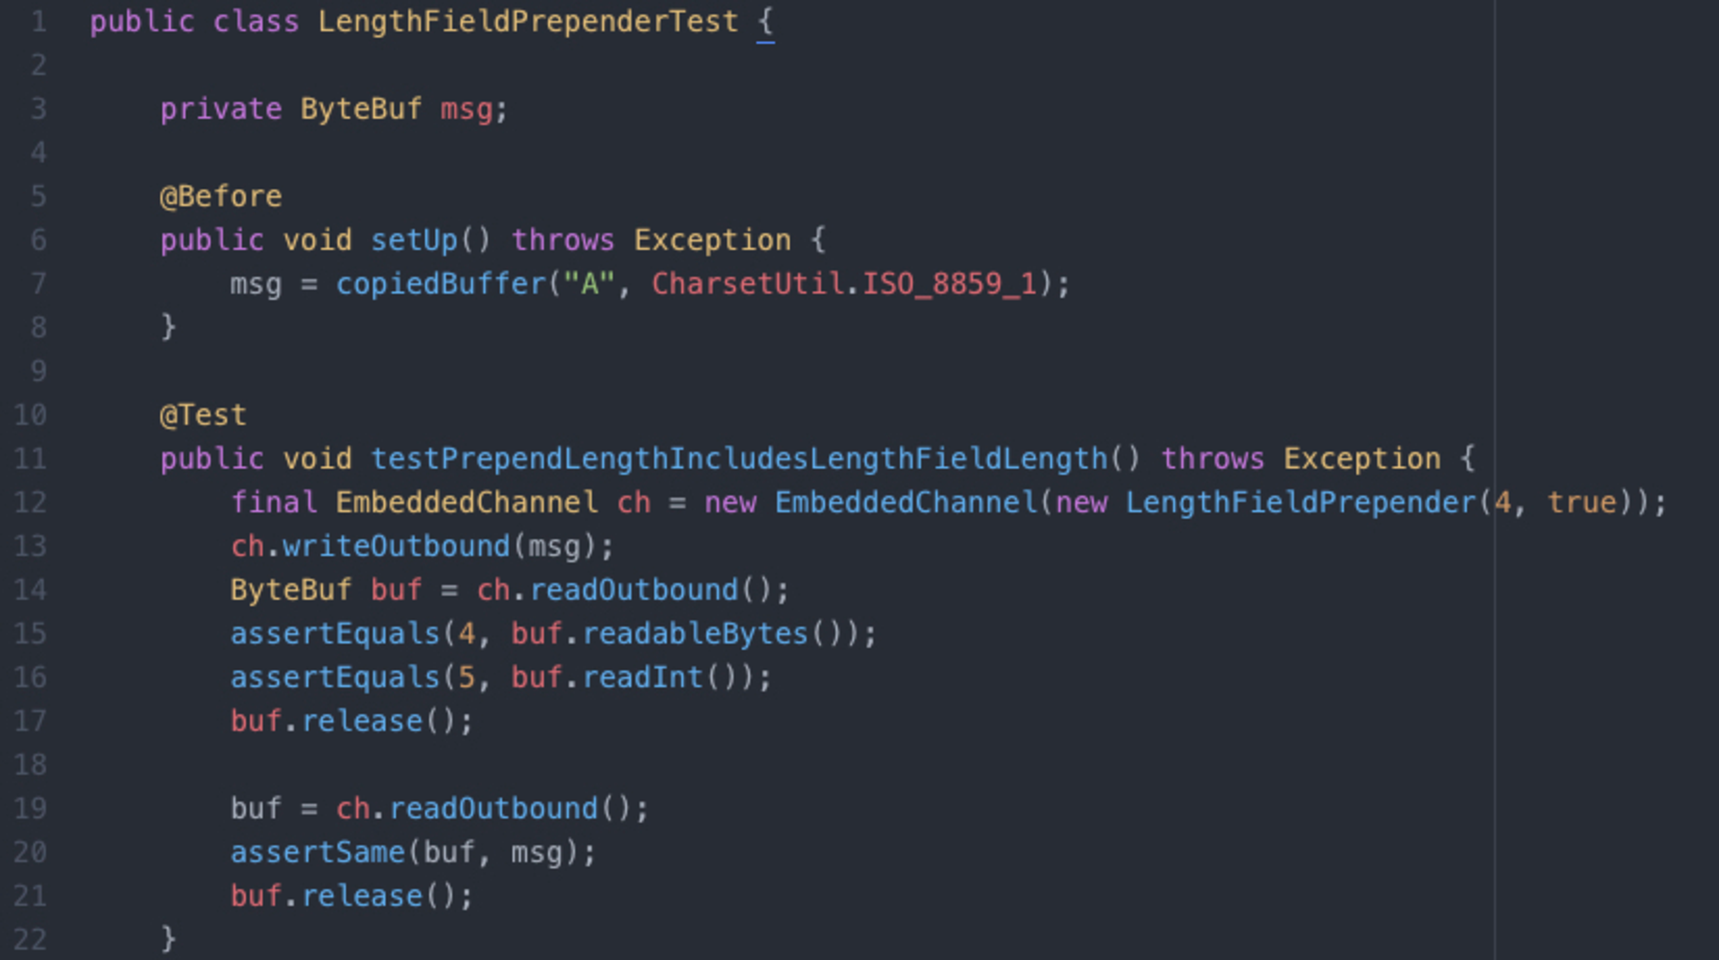
\includegraphics[width=14cm]{img/snipetB.pdf}
\caption{比較的複雑なテストコード例}
\label{snipetB}
\end{center}
\end{figure*}

より複雑なテストコード例として、nettyプロジェクトのLengthFieldPrependerTest.javaを図\ref{snipetB}に掲載する。
これも同様にJUnit4フレームワークが使用されており、@Testアノテーションが付与されたtestPrependLengthIncludesLengthFieldLengthメソッド(10行〜22行)がテストメソッドとして認識される。
nettyはJavaで非同期通信を行うアプリケーションを開発するためのオープンソースフレームワークである。
LengthFieldPrependerTestクラスはメッセージの長さを付加するエンコーダであるLengthFieldPrependerクラスを主にテストする。
LengthFieldPrependerのコンストラクタに第二引数としてTrueを与えることで、メッセージの長さに第一引数で指定した数を加算することができる。
testPrependLengthIncludesLengthFieldLengthメソッドはこの場合のテストシナリオを実現する。

このテストクラスには@Beforeアノテーションが付与されたsetUpメソッドが存在している。
JUnit4では全てのテストメソッドの実行前に@Beforeアノテーションが付与されたメソッドを実行する規則を持つ。
したがってtestPrependLengthIncludesLengthFieldLengthメソッドの実行前には常にsetUpメソッドが実行され、変数msgには文字列"A"が格納されている。

またこのテストメソッドは3つのアサーションを有している。
一つ目(15行)はエンコード後のバイト列に付加されたバイト数が指定した4であるかを検証する。
二つ目(16行)はエンコード後のバイト列が文字列"A"の長さ1に指定した4を付加した5であるかを検証する。
三つ目(20行)はエンコード後にデコードしたものが元のものと同一であるかを検証する。



\section{テストメソッド移植可能条件}

本章では、我々の提案するテストメソッド移植可能条件について説明する。
前提として、テストメソッドが移植可能であるとは、あるプロジェクトに属するテストメソッドが、それが依存する他のテスト補助メソッドと共に、メソッド名やクラス名などの識別子のみを変更した状態で別のプロジェクトに移動した場合に、コンパイルエラーを引き起こすことなく、その成否を問わずテストが正常に実行できることを指す。
テストメソッドの移植可能性はそれのみでは判断できず、ある移植元プロジェクトからある移植先プロジェクトに移植を行う上での移植可能性として判断される。

テストコードはプロダクトコードとは独立したものとして開発される。そのプロジェクトの提供したい機能はプロダクトコードによって実現され、テストコード自体はプロジェクトの機能実現に与しない。そのため、テストコードとプロダクトコードは適切に分離されており、プロダクトコードの一切の機能はテストコードに依存しない。このことから、テストコードからプロダクトコードのメソッドが呼び出されることはあるが、プロダクトコードからテストコードのメソッドが通常呼び出されることはない。従って、テストコードとプロダクトコード間の依存関係を調べるには、テストコード中に出現するプロダクトコードのメソッド呼び出しに注目すればよい。ここで、メソッド呼び出しにはクラスのインスタンス化を含む。

また、テストメソッド中のメソッドの呼び出しは以下の三種類に分類できる。

- A: Privateなメソッドなど、そのテストメソッドと同じクラス内に存在するメソッド、あるいは、別のテスト用のクラスに存在する補助メソッド。
- B: 外部からインポートしたライブラリに含まれるクラスのメソッド。
- C: テスト対象のプロダクトコードに含まれるクラスのメソッド。

このうち、Aはテストメソッドの移植に伴って同様に移植することでその依存関係を保つことができるため、移植可能条件には関与しない。またBも同様に、移植先で同じようにインポートすることで依存関係を保つことができるため、移植可能条件に関与しない。従って、テストメソッドの移植可能条件を考える際にはテストコード中に含まれるメソッド呼び出しのうち、Cのみを考えればよいことがわかる。

まず、最も厳格な移植可能条件は、移植元のプロジェクトにおいてテストメソッド中で呼び出される全てのCのメソッドおよびそれを所有するクラスがが移植先のプロジェクトにも存在していることである。

例えば、〜〜。

しかし、クラス名、およびメソッド名は、開発者が好きに命名できるものであり、それらがたまたま全て一致すると考えるのは現実的ではない。

前提の通り、テストメソッド中のテスト対象に依存するクラス名およびメソッド名はテスト対象である移植先リポジトリに存在するクラス名およびメソッド名に改変することが可能であると考えた場合、それが実行可能になる条件を考える。

条件1 テストメソッド中で呼ばれるプロダクトコードのメソッドと同じインターフェースを持つメソッドが全て移植先のプロジェクトに存在する

ここでインターフェースとは、メソッドが要求する引数の個数およびそれぞれの型、またメソッドの返す値の型を指す。

例えば、〜〜。

また引数あるいはメソッド自体の型をTとすると、Tの種類として次のパターンが考えられる。

- a: int, bool, longなど、Primitive型
- b: String, File, HttpSearverなど、外部からインポートしたライブラリで定義されたクラス型
- c: 移植するテストコードで定義されたクラス型
- d: 移植元のプロジェクトのプロダクトコードで定義されたクラス型

このうち、Tがaまたはcである場合、移植先でテストメソッドを移植することへの制限は特にない。
一方、Tがbであるメソッドmbを含むテストメソッドを移植しても実行が可能であるためには、移植先にmbと同じインターフェースを持つメソッドmb'を定義しているプロダクトコードが、bをインポートしている必要がある。
また、Tがdであるメソッドmdを含むテストメソッドを移植しても実行が可能であるためには、移植先にmdと同じインターフェースを持つメソッドmd'を定義しているプロダクトコードが移植先プロジェクトに存在する必要がある。

特にTがdである場合、移植元のプロダクトコードで定義されているクラスが移植先のプロダクトコードでも定義されていると考えるのは現実的ではない。
このことから、移植するテストメソッドに含まれる移植先プロダクトコードのメソッド`m`の呼び出しを移植先プロジェクトのプロダクトコードに含まれるメソッド`m'`に置き換える場合、次の条件を満たす必要がある。

条件2 `m`と`m'`が型として扱うテスト対象のプロダクトコード内で定義されたクラスは、そのテストメソッドが使用する範囲において、同じ役割を持つ。

例えば、〜〜。

ただし、テストメソッド中で呼び出されるメソッドで型として扱われるプロダクトコードで定義されたクラス間の関係は移植先でも保たれる必要がある。

\section{調査結果}

\subsection{RQ1}
\textbf{研究設問:テストコードの移植元として使用できるプロジェクトはどの程度存在するか?}

この研究設問に回答するため、GitHub\cite{GitHub}に存在するテストコードを持つJavaリポジトリについて調査する。

GitHubリポジトリデータを保管するサービスであるGHTorrent\cite{Gousios2013}とGitHubが提供するGitHub API\cite{GitHubAPIv3}を使用して全てのリポジトリの中から絞り込みを行う。
実験開始時に最新のものであった2019年6月末に登録されたGHTorrentのダンプデータから、主な言語がJavaであり、フォークによって作られたものではなく、リポジトリが削除されておらず、スターを100以上持つ11,464件のリポジトリ情報が得られた。
次にGitHub API v3を使用し、リポジトリのディレクトリ構造が記されたTreeオブジェクトを参照することで、テストコードであることが期待される、masterブランチにおいてtestディレクトリ下に存在する.javaファイルの数を調査した。
このファイル数が20以上である2,170件のリポジトリについて、2019年11月15日時点でのリポジトリをダウンロードした。またブランチがmasterでないものはmasterブランチに切り替えた。リポジトリの重複を排除し、ダウンロードおよびブランチの切り替えに成功したリポジトリは2,124件であった。

ここまではあくまでテストコードと期待できるファイルの存在によって絞り込みを行なっているため、ファイルの内容を確認して実際のテストコードを特定し、さらに絞り込む。
本実験では、テストフレームワークによって提供されるテストメソッドを持つコードファイルをテストコードと定義する。
テストメソッドの識別ルールはテストフレームワークによって異なり、メジャーなものでは以下の通りである。
\begin{itemize}
\item JUnit3:org.junit.TestCaseを継承したクラスのメソッドである。
\item JUnit4:メソッドに@Testアノテーションが付いている。
\item JUnit5:メソッドに@Test, @RepeatedTest, @ParameterizedTest, @TestFactory, @TestTemplateのいずれかのアノテーションが付いている。
\item TestNG:メソッドに@Testアノテーションが付いている。
\end{itemize}

JUnitやTestNGを使わずにマイナーなフレームワークや自作のテスト環境を使っている場合もあることは予想されるが、それらを自動的に識別することは難しいため、本研究では取り扱わない。

ファイルパスに/test/が含まれ、上述した条件を満たすメソッドを持つJavaコードファイルをテストコード、ファイルパスに/test/が含まれるが上述の条件を満たさないものをテスト補助コード、ファイルパスに/test/が含まれないJavaコードファイルをプロダクトコードに分類する。
Javaソースコードの静的解析にはJavaParserのPythonラッパーであるjavalangパッケージを使用した。

現段階で、2,124件のリポジトリが存在している。まず、Javaソースファイルが全く含まれていない4件のリポジトリを除外した。これらはGHTorrentおよび
GitHub APIによる絞り込みからリポジトリのダウンロードの間に大きな変更があったものである。

次に、全てのJavaファイルに対してPythonによる分析を行う上で、ファイルオープンの失敗、文字列へのデコードの失敗、javalangによるASTへのパースの失敗が確認されたファイル数を調査した結果、損傷ファイルを1つ以上持つリポジトリが687件存在した。
デコードの失敗原因は外字の使用、パースの失敗原因は構文エラーが考えられる。ファイルオープンに失敗したファイルは存在しなかった。
こうした損傷ファイルは以降の調査対象として扱うことができない。少量の損傷ファイルであればその存在を無視できるが、ファイル間の対応関係を扱う以上、無視すべきファイル数が多いと妥当性が損なわれるおそれがある。
全Javaファイルの5\%以上が損傷ファイルである37件のリポジトリを除外し、またその上で、損傷ファイル数が20以上であるリポジトリ53件を除外した。

次に、全てのJavaコードファイルの内容を調べ、org.junitまたはorg.testngを含むライブラリをインポートしているファイルが全く存在しない79件のリポジトリを除外した。

次に、分類の結果、プロダクトコードが0ファイルとなった6件のリポジトリを全て除外した。またその上で、テストコードが0ファイルとなった3件のリポジトリを除外した。

最後に、以降の実験のためにできるだけテストコードを多く持つリポジトリを扱いたいという目的から、分類の結果、テストコード数が10ファイル未満となった81件のリポジトリを除外した。

これらのフィルタリングによって最終的に1,862件のリポジトリが得られた。これらの統計情報について表\ref{tab:repos}に示す。

\begin{table}[t]
  \caption{ファイルタリング後の1,862リポジトリの情報}
  \label{tab:repos}
  \centering
  \begin{tabular}{lrrrr} 
    \hline
   (単位:個) & min. & ave. & mid. & max \\ \hline
    スター数 & 100 & 1,121.6 & 329 & 81,817 \\
    全Javaファイル & 22 & 898.3 & 338 & 57,851 \\
    テストコード & 10 & 156.3 & 58 & 3,508 \\
    プロダクトコード & 1 & 676.7 & 233 & 57,372 \\
    テスト補助コード & 0 & 65.0 & 15 & 3,371 \\ \hline    
  \end{tabular}
\end{table}

テストコードの移植を行う上では、移植先と同じドメインに属するリポジトリから移植できるテストコードを探すことが有効であると考えられる。
フィルタリングしたリポジトリのそれぞれに対して著者が手動でドメインのラベル付けを行なった。
Awesome Java[要引用]で用いられている66種類のドメイン名を参考に21種類のドメイン名に分類した。
各リポジトリのGitHubページのdescriptionおよびREADME.mdを確認することで、それが属すると思われるドメインを3つまで選択した。
ドメインに繋がる情報が得られないものや判断がつかないものに対してはNo Categoryとした。

ドメイン分類の結果を表\ref{tab:domain}に示す。
各ドメイン毎にそのラベルが貼られたリポジトリ数を示しているため、合計が総リポジトリ数と異なることに注意せよ。
ソフトウェア開発に用いられることを示すDevelopmentドメインを持つリポジトリが最も多かった。
次いで、データの処理や規格を扱うことを示すDataドメインやWebアプリケーションであることを示すWebドメインが多かった。
また、二つ以上のドメインの組み合わせで最も多かったものはDevelopmentとWebであった。

\begin{table}[t]
  \caption{ドメイン分類結果}
  \label{tab:domain}
  \centering
  \begin{tabular}{lr|lr} 
    \hline
domain & repositories & domain & repositories \\ \hline
Development & 339 & Multimedia & 100 \\
Data & 304 & Testing & 92 \\
Web & 256 & Security & 71 \\
Network & 201 & Document & 65 \\
Distribution & 159 & Performance & 46 \\
Database & 157 & OS & 44 \\
Programing & 137 & Financial & 41 \\
Operation & 135 & Geospatial & 31 \\
Android & 119 & Middleware & 30 \\
Utility & 104 & Game & 29 \\
Science & 101 & No Category & 54 \\ \hline
  \end{tabular}
\end{table}


\subsection{RQ2}
\textbf{研究設問:テストメソッドの持つ他のメソッドへの結びつきはどの程度存在するか?}

この研究設問に回答するため、リポジトリ中のテストメソッド中のメソッド呼び出し状況を調査する。
簡単化のため、これ以降の実験ではRQ1の調査で得られた1,862件のリポジトリのうち、上位6つのドメインであるDevelopment, Data, Web, Network, Distribution, Databaseに属するリポジトリを、それぞれスター数の多い順に100件選択して使用する。
ドメイン間にはリポジトリの重複が含まれるため、使用されるリポジトリの数は合計で508件となった。

リポジトリ内のJavaソースコードに対して静的解析を行い、メソッドの分類をおこなった。
またテストメソッド中で呼び出されているメソッドを調べ、その呼び出し先を分類した。
結果を以下に示す。

まず、リポジトリに存在するテストメソッドについての調査結果を述べる。
508件のリポジトリにおいて、ソースコードは合計548,595個存在し、そのうちテストコードは97,488個存在している。
これは全ソースコードのうち17.7\%を占める。
またメソッドは合計4,353,060個存在しており、
このうちテストメソッドは576,125個存在し、13.2\%を占める。
またプロダクトメソッドの総数は3,306,585個、テスト補助メソッドの総数は508,203個であった。
このことから、平均するとリポジトリに含まれるテストコードの量はプロダクトメソッドのおよそ1/6であり、テスト補助メソッドとはおよそ同数となる。
加えて1つのリポジトリあたりに含まれるテストメソッド数の平均値は1134.1個、中央値は785.0個であった。
また1つのテストコードあたりに含まれるテストメソッド数の平均値は5.9個、中央値は3.0個であった。


\begin{figure}[tb]
\begin{center}
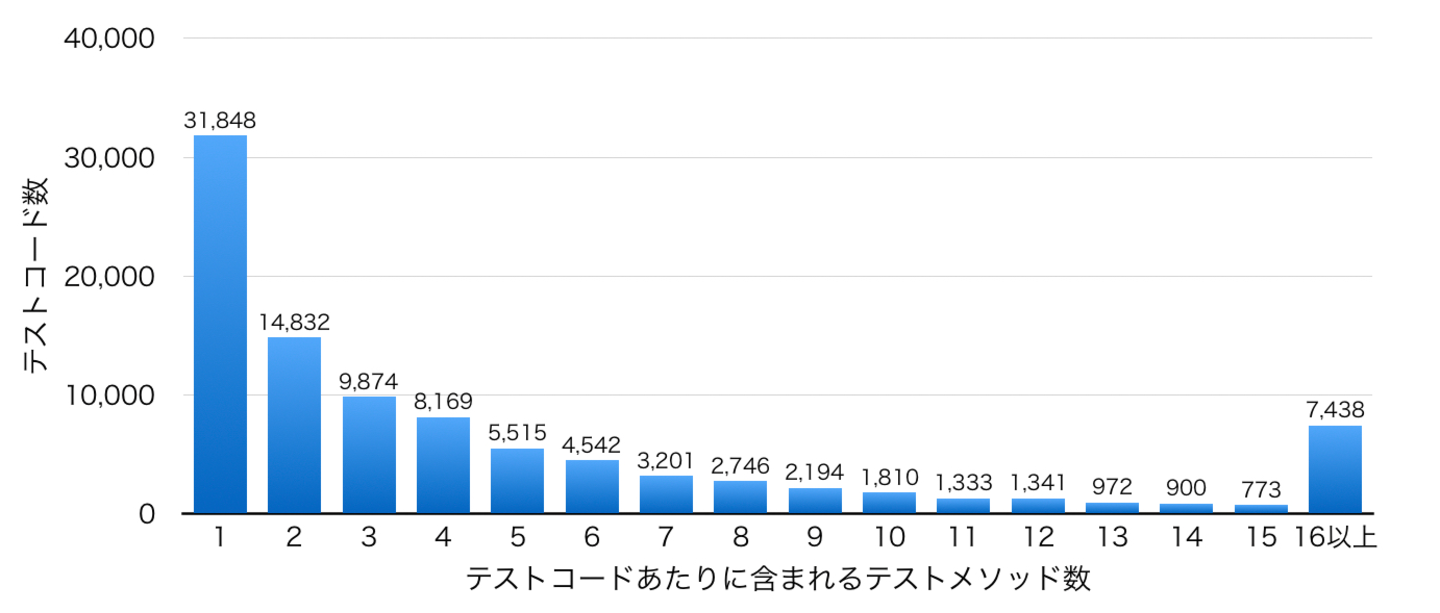
\includegraphics[width=8.5cm]{img/testcodes.pdf}
\caption{テストコードあたりに含まれるテストメソッド数のヒストグラム}
\label{testcodes}
\end{center}
\end{figure}

テストコードあたりに含まれるテストメソッド数の分布について図\ref{testcodes}のヒストグラムに示す。
テストメソッドを1つのみ含むテストコードが最も多く、テストメソッド数が増えるごとにそれを含むテストコード数が少なくなっていくが、16個以上といった多くのテストメソッドを含むテストコードもまた多く存在していることがわかる。

\begin{table}[t]
  \caption{テストメソッド内で呼び出されるメソッドについて}
  \label{tab:called}
  \centering
  \begin{tabular}{lrrr} 
    \hline
   (単位:個) & ave. & mid. & std. \\ \hline
    テストメソッドが呼び出すメソッド数& 5.7 & 4.0 & 7.3 \\
    テストシナリオが直接呼び出すメソッド数 & 8.3 & 5.0 & 11.0 \\
     プロダクトメソッド & 2.6 & 1.0 & 4.4 \\
     テスト補助メソッド & 0.8 & 0 & 1.8 \\
     外部ライブラリメソッド & 4.6 & 2.0 & 6.8 \\
    テストシナリオが結果的に呼び出すメソッド数 &  &  &  \\
     プロダクトメソッド & 2.8 & 1.0 & 4.1 \\
     テスト補助メソッド & 1.0 & 0 & 2.4 \\
     外部ライブラリメソッド & 8.9 & 3.0 &22.6 \\ \hline
  \end{tabular}
\end{table}

次に、テストメソッド内で呼び出されるメソッドについての調査結果を述べる。
これらの結果については表\ref{tab:called}にまとめている。
一つのテストメソッドの中では、同一メソッドの重複を排除すると、平均5.7個のメソッドが呼び出されていることが分かった。
また2章で説明したように、テストメソッドの実行に伴って実行される@Beforeあるいは@Afterアノテーションを持つメソッドの一続きの実行を以降テストシナリオと呼ぶ。
一つのテストシナリオの中では、平均8.3個のメソッドが呼び出されていることが分かった。
これらの呼び出されるメソッドの呼び出しは、プロダクトメソッドが平均2.6個、テスト補助メソッドが平均0.8個、外部ライブラリのメソッドが平均4.6個と分類できる。
外部ライブラリメソッドの呼び出しは、例えばJUnitの提供するアサーションを行うメソッドや、文字列を扱うStringクラスの汎用的なメソッドなどが多く該当する。

テストメソッドが呼び出したテスト補助メソッドの中で、さらにメソッド呼び出しを行う場合、それらもテストシナリオが呼び出すメソッドに含まれているとみなすことができる。
こうした再起的なメソッド呼び出しも考慮して集計した結果、一つのテストシナリオは平均12.7個のメソッドを結果的に呼び出していることが分かった。
これらはプロダクトメソッドが平均2.8個、テスト補助メソッドが平均1.0個、外部ライブラリのメソッドが平均8.9個と分類できる。
テスト補助メソッド内の呼び出しを考慮しても、プロダクトメソッドの新たな呼び出しはほとんど行われず、外部ライブラリの呼び出しが増える傾向にある。

この結果から次のことが言える。
あるプロジェクトに存在するあるテストシナリオを別のプロジェクトに移植する場合、それはテスト対象となるプロダクトに対して平均2.8個のメソッド呼び出しを通じて依存している。
したがって、平均2.8個のメソッドについて、移植元のプロジェクトと移植先のプロジェクトの間でメソッドの対応付けが必要となる。
またテストシナリオの移植に伴って、平均1つのテスト補助メソッドも同時に移植する必要がある。
さらに外部ライブラリから平均8.9個メソッドを利用するため、これらのライブラリを準備する必要がある。

TODO; これらのメソッドが属するクラスはいくつあるのか

TODO; 依存するプロダクトメソッドについて、引数の数と種類を分類



\subsection{RQ3}

\subsection{RQ4}

\section{discussion}

\section{Thread to validity}
\subsection{Internal Validity}
自作ツールの動作が正しくないかもしれない

ドメイン分類が妥当じゃないかもしれない

調査時期にズレがある

\subsection{External Validity}
508個のリポジトリの内容しか見ていないので一般化できないかもしれない

30個のリポジトリに対してしかテストメソッド移植の評価をしていないので一般化できないかもしれない

\subsection{Construct Validity}
実行可能性を保つことしか見てないのでちゃんとテストできないかもしれない

スターが100以上やテストコードらしきファイルの数が20個以上などの基準は著者が目安として定めたものなので妥当ではないかもしれない。

\section{Related work}
\subsection{テストコード自動生成}
ソースコードからテストコード
EvoSuite\cite{Fraser2013}
Randoop\cite{Pacheco2007}

自然言語からテストコード
JDoctor\cite{Arianna2018}
Toradacu\cite{Alberto2016}
@tComment\cite{Tan2012}

BDD自動変換

\subsection{ソースコード再利用}
Program Splicing\cite{Lu2018}
\subsection{テストコード解析}

\section{Conclusion}
本研究では、再利用によるJavaテストコードの自動生成手法の提案に向け、テストコードの移植が可能となる条件を提案し、既存プロジェクトにおけるテストコードの移植可能性について調査した。
GitHubに存在するテストコードを持つリポジトリを選定し調査した結果、一つのリポジトリから移植元として利用できるテストメソッドが平均1,000個程度得られることや、

今後の課題として、
が挙げられる。


\bibliographystyle{IEEEtran}
\bibliography{reference}

\end{document}


